\documentclass[preprintnumbers,aps,prd,floatfix,nofootinbib,onecolumn]{revtex4}
\usepackage{epsfig}
\usepackage{graphicx}
\usepackage{url,hyperref}
\usepackage{bm}
\usepackage{float}
\usepackage{amsmath}
%opening
%\title{Sample phase space EQ}
%\author{jogh}

\begin{document}
\maketitle
\section{Speed of Expert Agreement}
In these simulations there are 10 experts, with the initial settings given by
\begin{align}
&d_i^{\text{initial}}={}\{1,0,-1,-2,-2,1,0,-1,-2,-2\}\,,\qquad h=0.99\nonumber
\end{align}
and at each given step (question), the values of affinity and bias are assigned as
\begin{align}
a_i={}&\{a,a,a,a,a,a,a,a,a,a\}\,,\qquad b_i={}\{0,0,b,b,b,0,0,b,b,b\}\,,\nonumber
\end{align}
where $a$ and $b$ are generated randomly in the interval $[0,10]$. For now, each simulation is independent so that each  diagram below shows different points in phase space (this to be fixed). The purpose of this simulation is to verify that the reward system tends to improve knowledge of the theory, in a reward-driven behaviour. Note that while all experts take the same value of  affinity  $a$, while it is assumed that only those experts who disagree with theory are biased. 
%\begin{figure}[H]
%\centering
%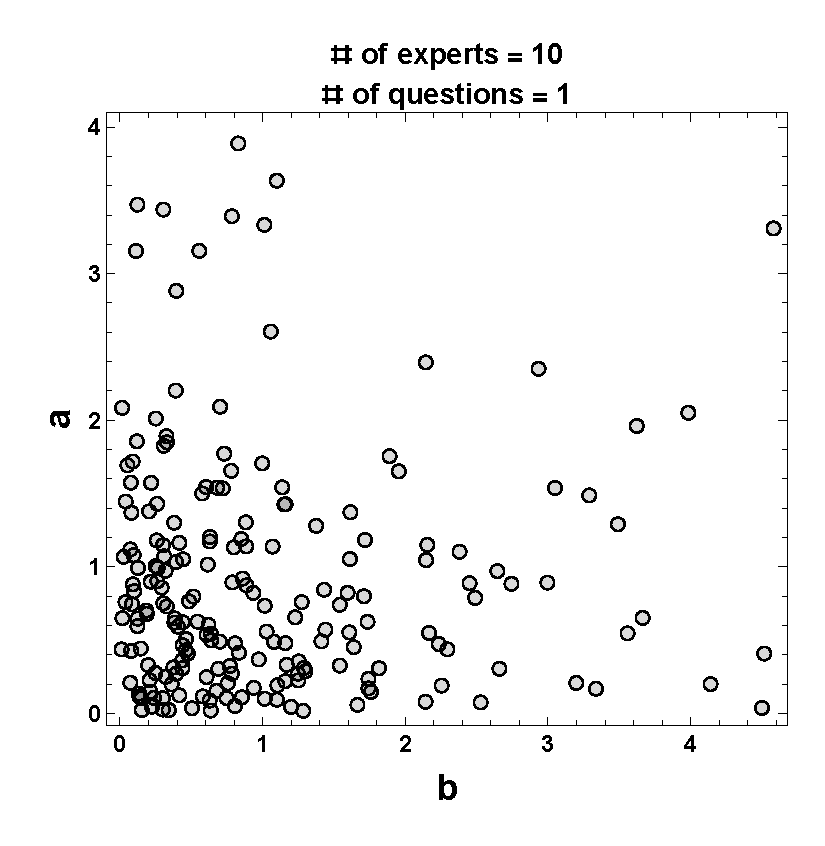
\includegraphics[width=0.4\textwidth]{../phase_q-1_1.pdf}
%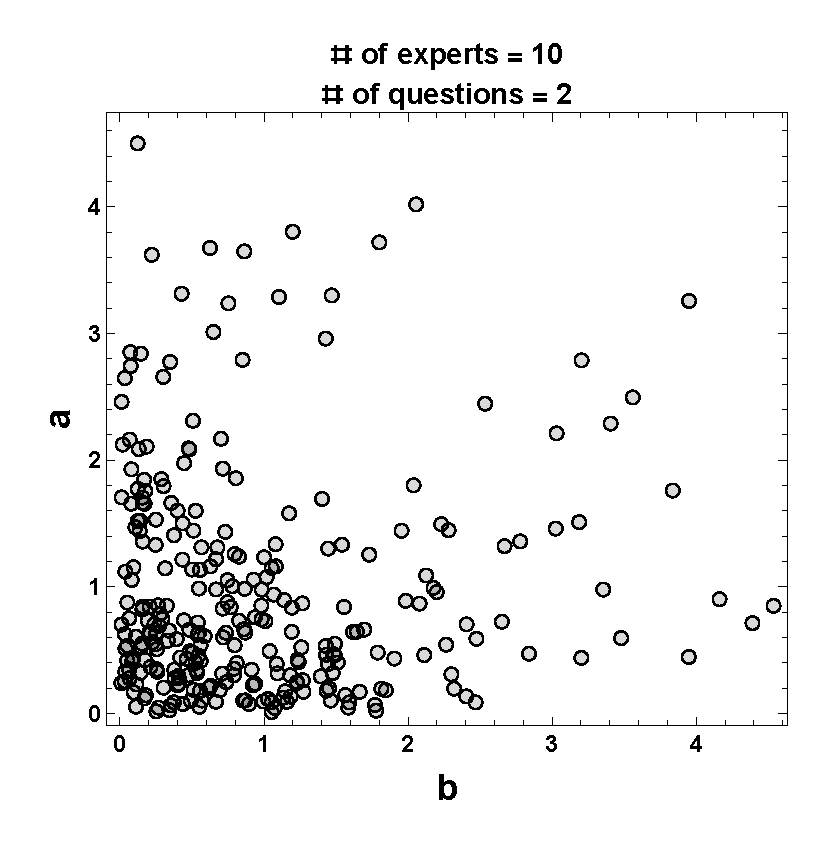
\includegraphics[width=0.4\textwidth]{../phase_q-2_1.pdf}
%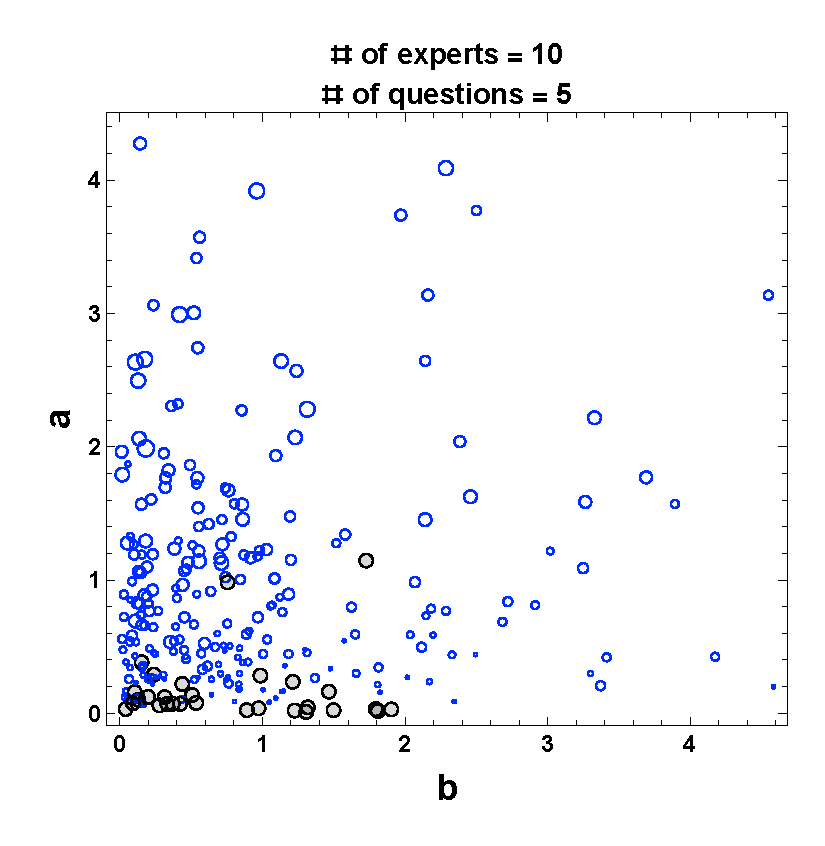
\includegraphics[width=0.4\textwidth]{../phase_q-5_1.pdf}
%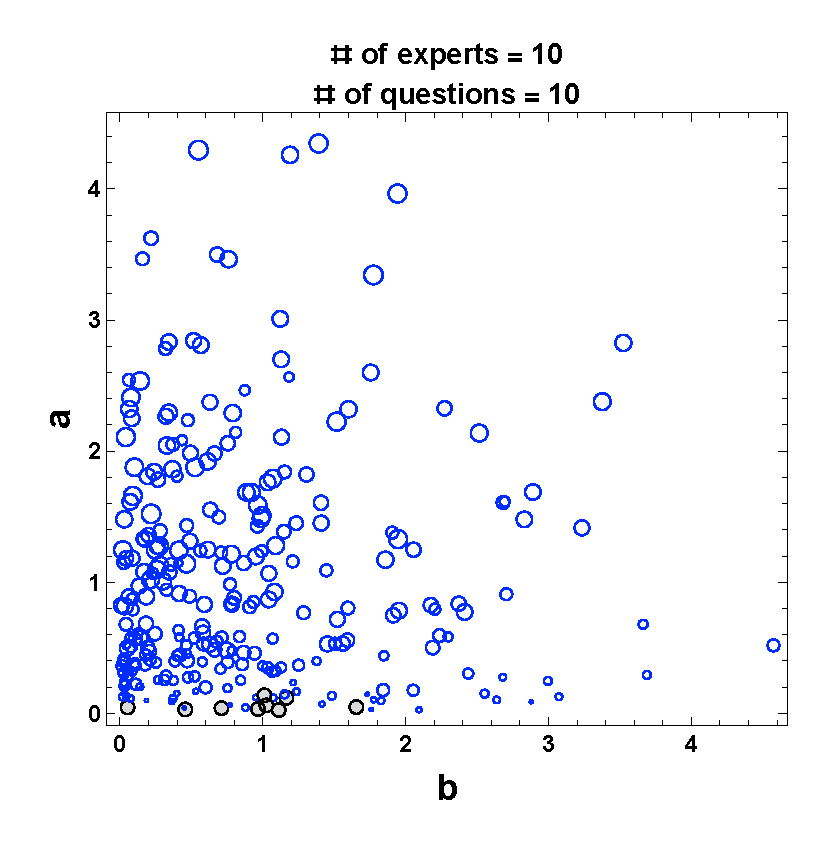
\includegraphics[width=0.4\textwidth]{../phase_q-10_1.pdf}
%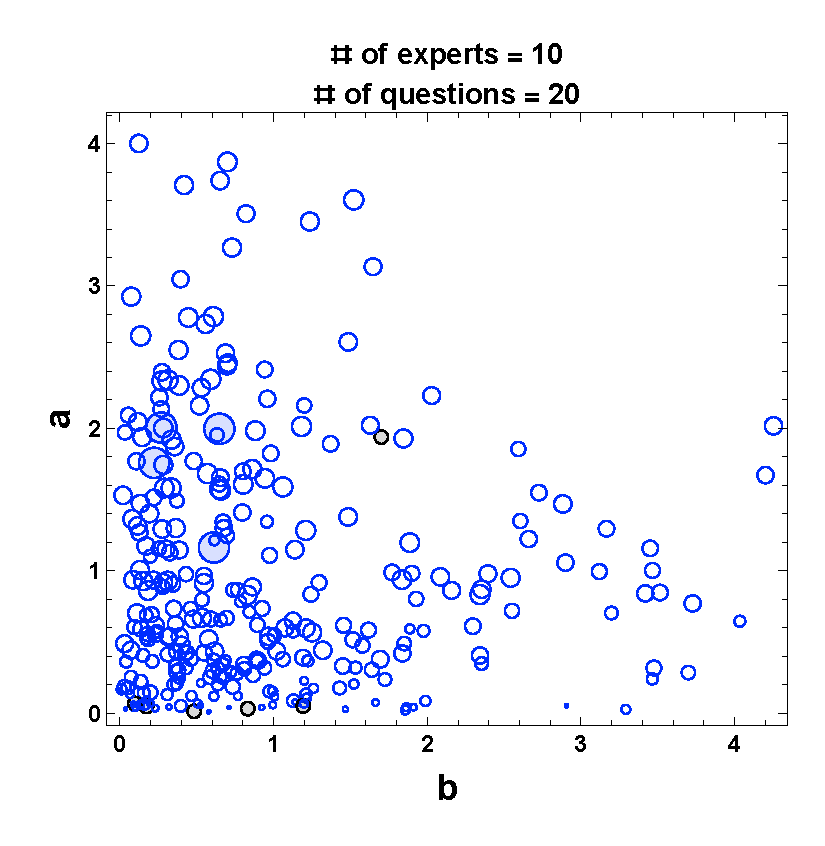
\includegraphics[width=0.4\textwidth]{../phase_q-20_1.pdf}
%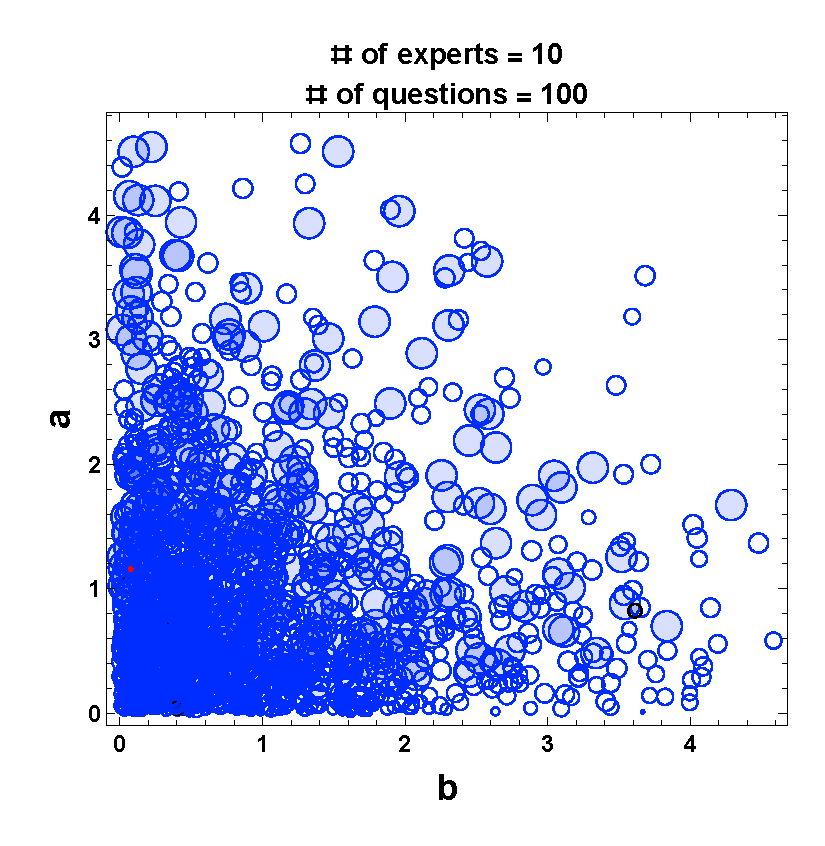
\includegraphics[width=0.4\textwidth]{../phase_q-100_1.pdf}
%\end{figure}
\begin{figure}[]
	\centering
	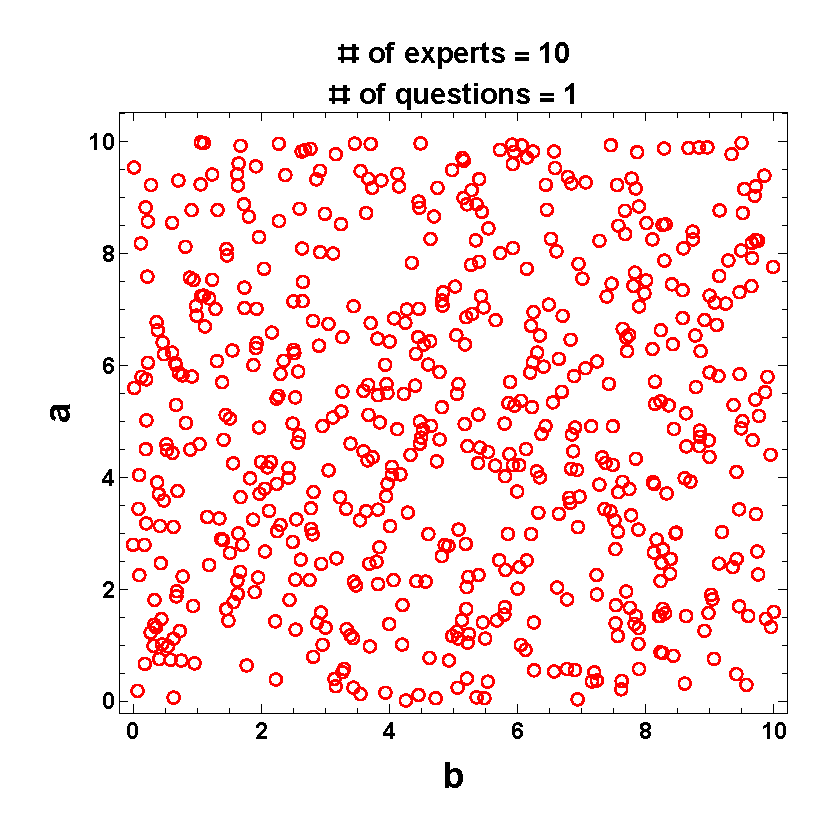
\includegraphics[width=0.4\textwidth]{../phase_try_red_q-1_1.pdf}
	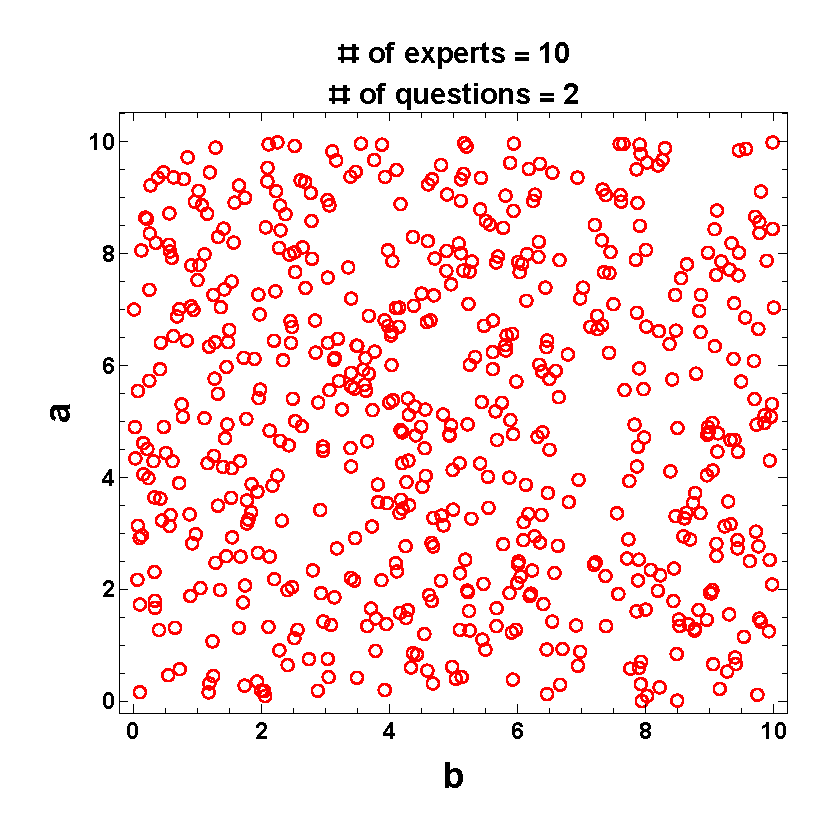
\includegraphics[width=0.4\textwidth]{../phase_try_red_q-2_1.pdf}
	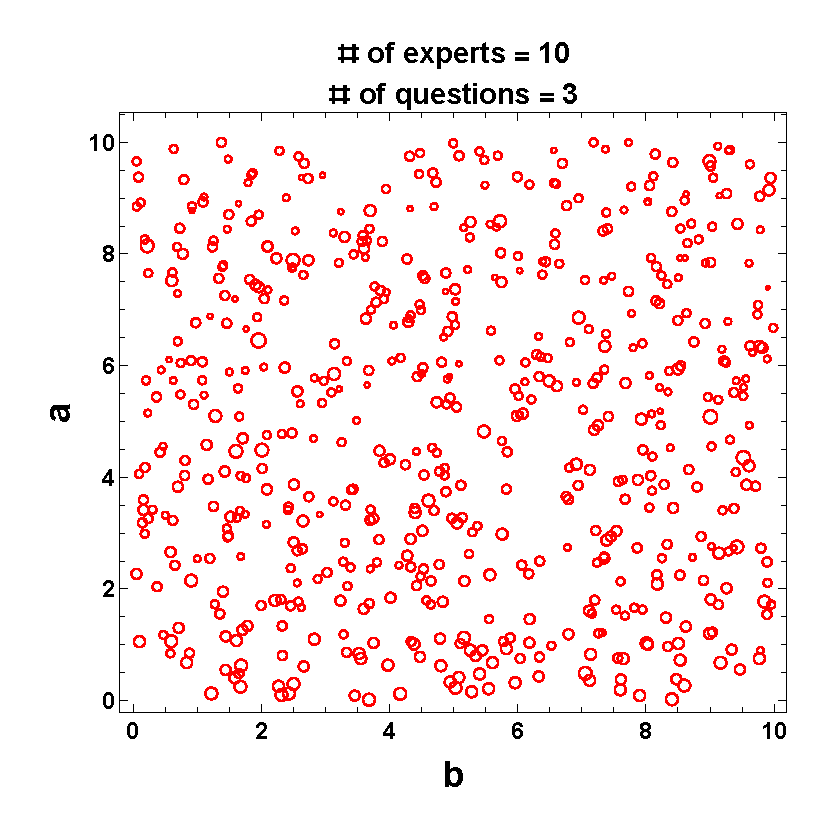
\includegraphics[width=0.4\textwidth]{../phase_try_red_q-3_1.pdf}
	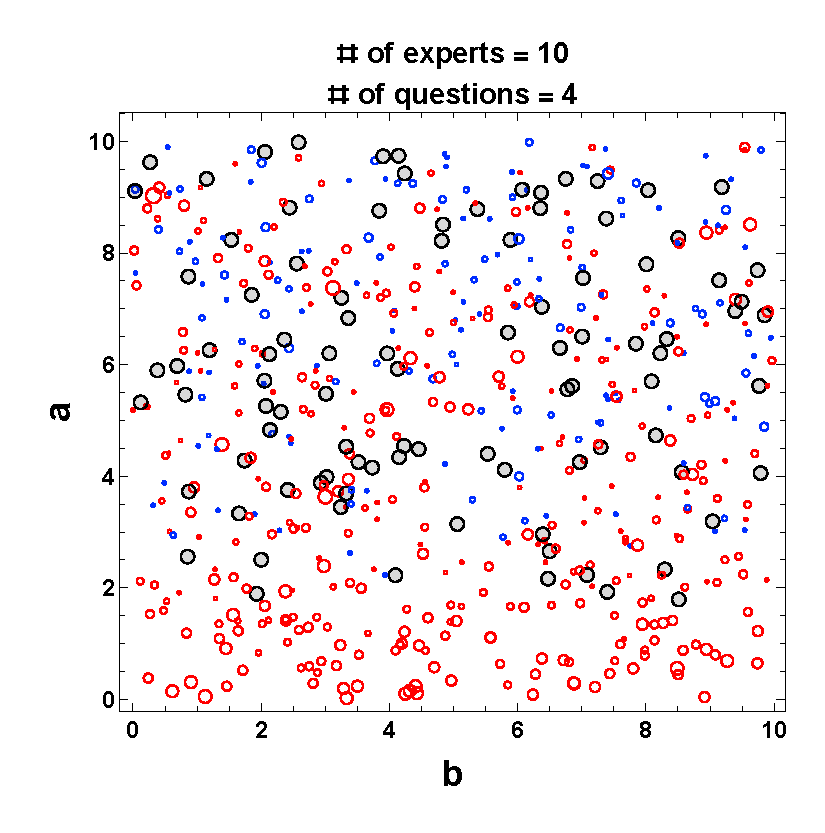
\includegraphics[width=0.4\textwidth]{../phase_try_red_q-4_1.pdf}
\end{figure}
\begin{figure}[]
	\centering
	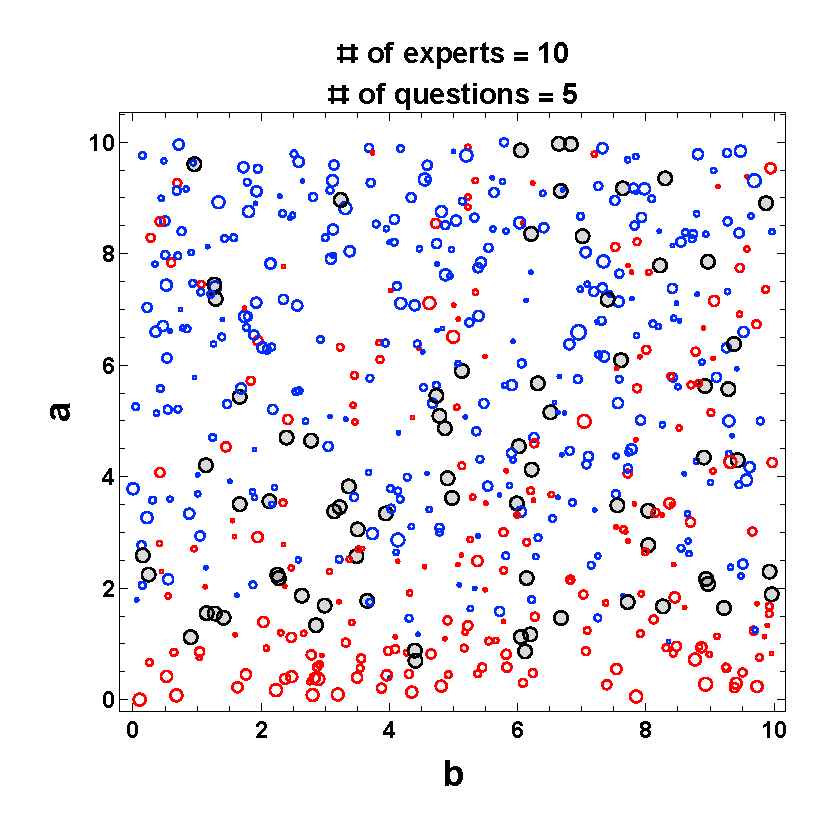
\includegraphics[width=0.4\textwidth]{../phase_try_red_q-5_1.pdf}
	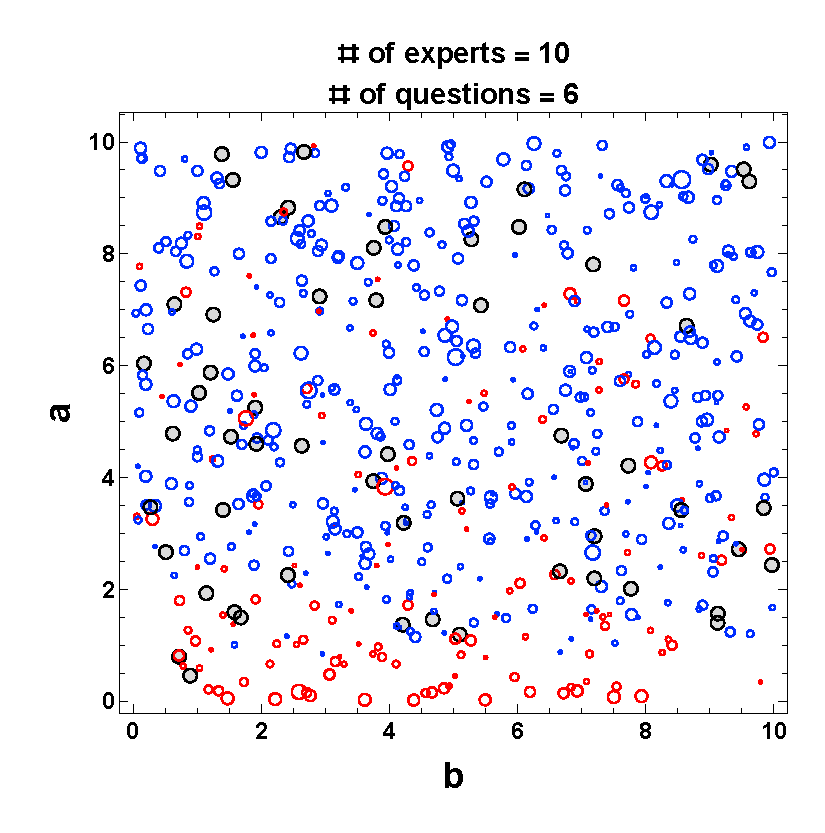
\includegraphics[width=0.4\textwidth]{../phase_try_red_q-6_1.pdf}
\end{figure}
\begin{figure}[]
	\centering
	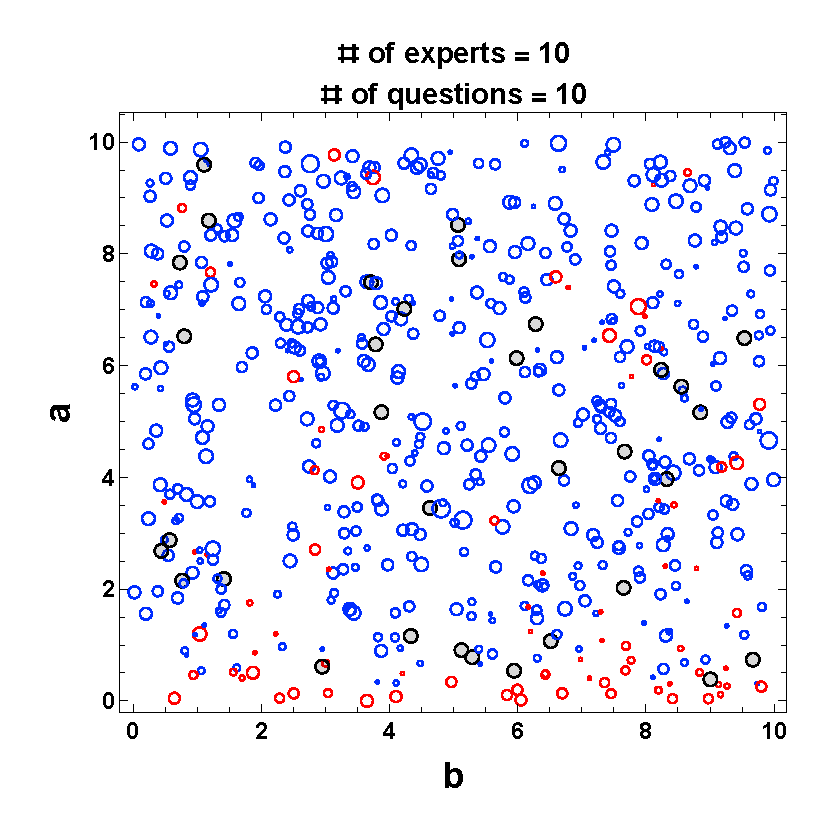
\includegraphics[width=0.4\textwidth]{../phase_try_red_q-10_1.pdf}
	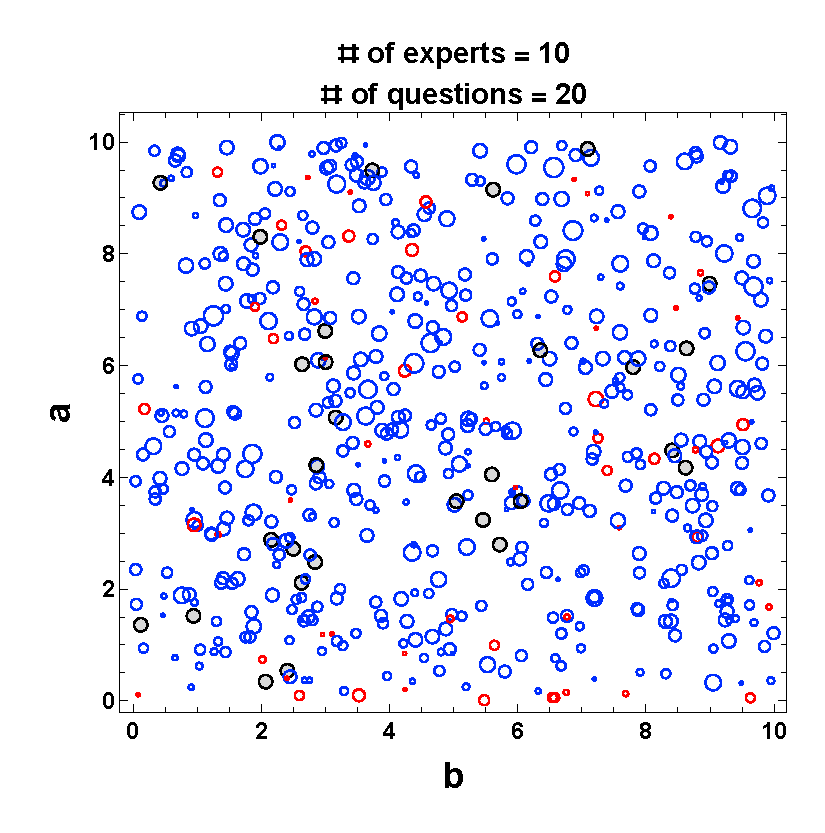
\includegraphics[width=0.4\textwidth]{../phase_try_red_q-20_1.pdf}
	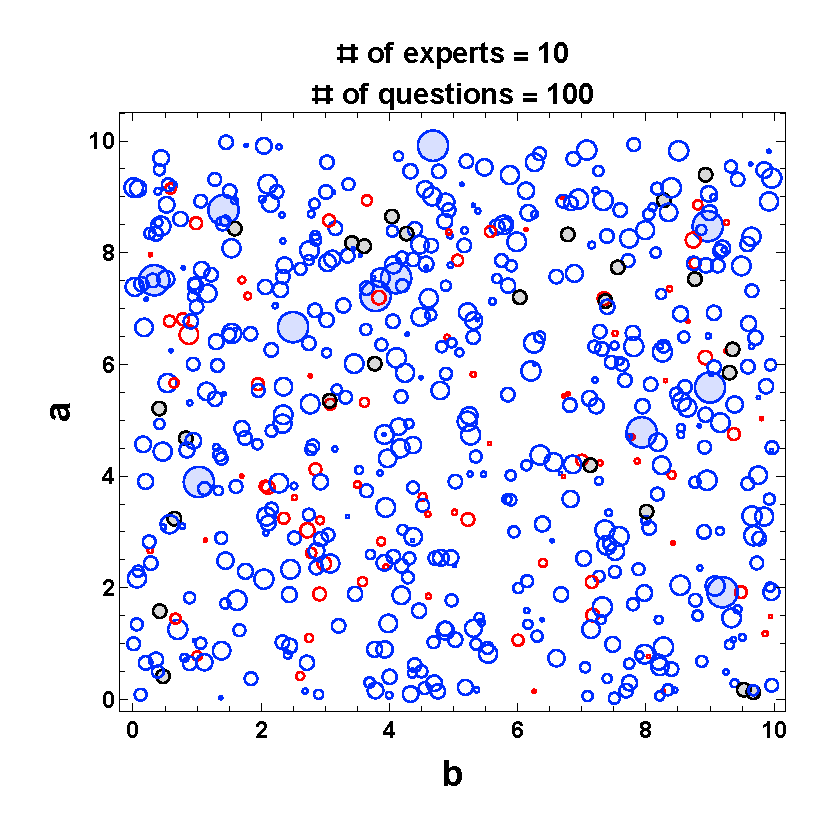
\includegraphics[width=0.4\textwidth]{../phase_try_red_q-100_1.pdf}	
\end{figure}


\end{document}
